\documentclass[../../notes.tex]{subfiles}

\pagestyle{main}
\renewcommand{\chaptermark}[1]{\markboth{\chaptername\ \thechapter\ (#1)}{}}
\stepcounter{chapter}

\begin{document}




\chapter{Basic Topology}
\section{Notes}
\begin{itemize}
    \item \marginnote{11/1:}Equivalence relationships are denoted $A\sim B$.
    \begin{itemize}
        \item These are\dots
        \begin{itemize}
            \item Reflexive ($A\sim A$).
            \item Symmetric ($A\sim B\Longleftrightarrow B\sim A$).
            \item Transitive ($A\sim B\ \&\ B\sim C\Longrightarrow A\sim C$).
        \end{itemize}
        \item Equivalence relations give rise to equivalence classes.
    \end{itemize}
    \item \textbf{Countable} (set $A$): A set $A$ such that $A\sim\N$, in the sense that there exists a one-to-one and onto map from $\N\to A$.
    \begin{itemize}
        \item Alternatively, $A$ can be written in the form $A=\{f(n):n\in\N\}$.
    \end{itemize}
    \item \textbf{Finite countable} vs. \textbf{infinite countable} (see \textcite{bib:Rudin}).
    \item $\N$ denotes the natural numbers.
    \item $\N_0$ denotes the natural numbers including 0.
    \item $\Z$ denotes the integers.
    \item We know that $\N\sim\Z$: Let $f:\N\to\Z$ be defined by
    \begin{equation*}
        f(n) =
        \begin{cases}
            \frac{n}{2} & n\text{ even}\\
            \frac{n-1}{2} & n\text{ odd}
        \end{cases}
    \end{equation*}
    \item More facts.
    \begin{enumerate}
        \item Every subset of a countable set is countable.
        \item Unions of countable sets are countable.
        \begin{itemize}
            \item If the sets $E_n$ for some finite list of numbers are countable, then $\bigcup_nE_n$ is countable.
            \item Soug goes over the diagonalization method of counting.
        \end{itemize}
        \item $n$-fold Cartesian products of countable sets are countable (we induct on $n$).
        \begin{itemize}
            \item If $A$ is countable and $B$ is countable, then $A\times B$ is countable.
            \item If $A$ is finite and to each $\alpha\in A$ we assign a countable set $E_\alpha$, $\otimes_{\alpha\in A}E_\alpha$ is countable.
        \end{itemize}
    \end{enumerate}
    \item \textbf{Metric space}: A space $X$ along with a matrix $d:X\times X\to[0,\infty)$ such that
    \begin{itemize}
        \item $d(x,y)>0$ iff $x\neq y$, and $d(x,x)=0$ iff $x=0$.
        \item $d(x,y)=d(y,x)$.
        \item $d(x,y)\leq d(x,z)+d(z,y)$.
    \end{itemize}
    \item Example ($\R^n$):
    \begin{itemize}
        \item We may define $d$ by
        \begin{equation*}
            d(x,y) = \sqrt{\sum(x_i-y_i)^2}
        \end{equation*}
        \item We can also define the $p$-metrics (recall normed spaces) with $p$ where 2 is.
    \end{itemize}
    \item Example ($X_p=\{f:Y\to\R:1\leq p<\infty,\int_Y|f|^p\dd{y}<\infty\}$):
    \begin{itemize}
        \item This is $\ell_p$.
        \item Define
        \begin{equation*}
            \norm{f-g}_p = \left[ \int_Y|f-g|^p\dd{y} \right]^{1/p}
        \end{equation*}
    \end{itemize}
    \item Convergence: $x_n\to x\Longleftrightarrow d(x_n,x)\to 0$.
    \item \textbf{Neighborhood}: The set of all points a distance less than $r$ away from $p$. \emph{Denoted by} $\bm{N_r(p)}$. \emph{Given by}
    \begin{equation*}
        N_r(p) = \{q\in X:d(p,q)<r\}
    \end{equation*}
    \item \textbf{Limit point} (of $E$): A point $p$ such that every neighborhood of $p$ intersects $E$ at a point other than $p$. \emph{Also known as} \textbf{accumulation point}.
    \begin{itemize}
        \item Symbolically,
        \begin{equation*}
            N_r(p)\cap(E\setminus\{p\}) \neq \emptyset
        \end{equation*}
        for all $r>0$.
    \end{itemize}
    \item \textbf{Isolated point} (of $E$): A point $p$ such that $p\in E$ and $p$ is not a limit point of $E$.
    \item \textbf{Closed} (set $E$): A set $E$ that contains all of its limit points.
    \item \textbf{Interior} (point $p$): A point $p$ such that there exists $N_r(p)\subset E$.
    \item \textbf{Open} (set $E$): A set $E$, all points of which are interior points.
    \item \textbf{Perfect} (set $E$): A set $E$ that is closed and every point of $E$ is a limit point of $E$.
    \item \textbf{Bounded} (set $E$): There exists a number $M$ and a $y\in X$ such that $E\subset\{p:d(p,y)\leq M\}$.
    \item \textbf{Dense} (set $E$ in $X$): A set $E$ such that every point of $X$ is a limit point of $E$ or a point of $E$, itself.
    \item \marginnote{11/3:}Every neighborhood is an open set.
    \item If $p$ is a limit point of $E$, every neighborhood of $p$ contains infinitely many points of $E$.
    \begin{itemize}
        \item Thus, a finite set cannot have a limit point.
        \item Prove by contradiction: Suppose there is a neighborhood that contains only finitely many points of $E$. Then the neighborhood with radius smaller than the distance to the closest point does not contain any points of $E$, a contradiction.
    \end{itemize}
    \item $E$ is open iff $E^c$\footnote{The complement of $E$.} is closed.
    \begin{itemize}
        \item Assume $E^c$ closed. If $p\in E$, then $p$ is not a limit point of $E^c$. It follows that there exists a neighborhood of $p$ that is entirely contained within $E$, so $p$ is interior, as desired.
        \item Suppose $E$ is open. Let $p$ be any limit point of $E^c$. Then $p\in E^c$.
    \end{itemize}
    \item $F$ is closed iff $F^c$ is open.
    \item If $(G_\alpha)_{\alpha\in A}$ is a family of open sets in $X$, then the union is open.
    \begin{itemize}
        \item Let $p\in\bigcup_{\alpha\in A}G_\alpha$. Then $p\in G_\alpha$ for some $\alpha\in A$. It follows that $p$ is an interior point of $G_\alpha$, so thus an interior point of the union of $G_\alpha$ with everything else.
    \end{itemize}
    \item Finite intersections of open sets are open.
    \begin{itemize}
        \item In the infinite case $\bigcap_{n\in\N}(-1/n,1/n)=\{0\}$, an intersection of infinitely many open sets is closed.
        \item However, in the finite case, just consider the neighborhood with the smallest radius and take this one.
    \end{itemize}
    \item The intersection of closed sets is closed.
    \item The union of finitely many closed sets is closed.
    \begin{itemize}
        \item These follow from the previous two by De Morgan's rule.
    \end{itemize}
    \item Let $\bar{E}=E\cup E'$ where $E'$ is the set of limit points of $E$.
    \item Let $X$ be a metric space and $E\subset X$. Then
    \begin{enumerate}
        \item $\bar{E}$ is closed.
        \begin{itemize}
            \item WTS: $\bar{E}^c$ is open. Let $p\in\bar{E}^c$. Then $p$ is neither in $E$ nor is it a limit point of $E$. Thus, there exists a neighborhood of $\bar{E}^c$ containing entirely points of $\bar{E}^c$. Therefore, $\bar{E}^c$ is open, so $\bar{E}$ is closed.
        \end{itemize}
        \item $E=\bar{E}$ iff $E$ is closed.
        \begin{itemize}
            \item Think $p\in\bigcap G_\alpha$?
        \end{itemize}
        \item $\bar{E}\subset F$ for any closed $F\supset E$.
        \begin{itemize}
            \item If $E\subset F$, then any limit point of $E$ will be a limit point of $F$. Thus, $E'\subset F'$. Then $\bar{E}=E\cup E'\subset F\cup F'=\bar{F}=F$ where the last equality holds because $F$ is closed.
        \end{itemize}
    \end{enumerate}
    \item Types of sets.
    \begin{table}[h!]
        \centering
        \small
        \renewcommand{\arraystretch}{1.4}
        \begin{tabular}{l|c|c|c|c}
             & Closed & Open & Perfect & Bounded\\ \hline
            $\{z\in\Q:|z|<1\}$ & N & Y & N & Y\\ \hline
            $\{z\in\Q:|z|\leq 1\}$ & Y & N & Y & Y\\ \hline
            Nonempty finite set & Y & N & N & Y\\ \hline
            $\Z$ & Y & N & N & N\\ \hline
            $\{1/n:n\in\N\}$ & N & N & N & Y\\ \hline
            $\R^2$ & Y & Y & Y & N\\ \hline
            $(a,b)$ & N & ? & N & Y\\
        \end{tabular}
        \caption{Types of sets.}
        \label{tab:typesSets}
    \end{table}
    \item \textbf{Relatively open} (set $E$ to $Y$): A set $E\subset Y\subset X$ such that if $p\in E$, then there exists a $Y$-neighborhood of $E$ contained in $E$.
    \item Let $N_r^X(p)=\{y\in X:d(y,p)<r\}$ be a neighborhood of $p$ in $X$, and let $N_r^Y(p)=\{y\in Y:d(y,p)<r\}$ be a neighborhood of $p$ in $Y$. Then $N_r^Y(p)=N_r^X(p)\cap Y$.
    \item $E$ is open relative to $Y$ iff $E=G\cap Y$ where $G$ is open relative to $X$.
    \item Introduces the supremum.
    \item If $E\subset\R$, $E\neq\emptyset$, and $E$ is bounded above, $\sup E<\infty$.
    \item Let $y=\sup E$. Then $y\in\bar{E}$.
    \item There exists a sequence $a_n\in A$ such that $a_n\to x=\sup A$.
    \item $A$ is compact iff any open cover of the set has a finite subcover.
    \item Study and \emph{know} all of these proofs.
    \item \marginnote{11/5:}Compactness: Defines compactness in terms of open covers.
    \item Finite sets are compact.
    \item Compactness is "absolute" (i.e., it is not a relative property like openness).
    \begin{itemize}
        \item If $K\subset Y\subset X$, then $K$ is compact relative to $X$ iff $K$ is compact relative to $Y$.
        \item $V$ is open relative to $Y$ iff $V=G\cap Y$ where $G$ is open relative to $X$.
    \end{itemize}
    \item Compact implies closed.
    \begin{itemize}
        \item We will show $K$ compact implies $K^c$ open.
        \item WTS: For all $p\in K^c$, there exists $N_r(p)\subset K^c$ suh that $N_r(p)\cap K=\emptyset$.
    \end{itemize}
    \item A closed subset of a compact set is compact.
    \begin{itemize}
        \item Let $K$ be compact and let $F\subset K$ be closed.
        \item Take any open cover of $F$. Extend it to an open cover of $K$. Take the finite subcover of $K$. Naturally, this finite subcover is also a finite cover of $F\subset K$.
    \end{itemize}
    \item $F$ closed, $K$ compact implies $F\cap K$ compact.
    \item If $(K_\alpha)_{\alpha\in A}$ is compact in $X$ with finite intersection property (every intersection of any finite number of these sets is nonempty), then $\bigcap_{\alpha\in A}K_\alpha\neq\emptyset$.
    \begin{itemize}
        \item Argue by contradiction.
        \item Let $G_\alpha=K_\alpha^c$.
        \item Assume the intersection is empty. Assume WLOG that no point of $K_1$ is in any of the other $K_\alpha$'s.
        \item Then $\{G_\alpha\}_{\alpha\in A}$ be an open cover of $K_1$.
        \item $K_1$ compact implies there is a finite subcover $G_{\alpha_1},\dots,G_{\alpha_n}$. Then $K\subset G_{\alpha_1}\cup\cdots\cup G_{\alpha_n}$. This implies that $K_1\cap K_{\alpha_1}\cap\cdots\cap K_{\alpha_n}=\emptyset$, a contradiction.
    \end{itemize}
    \item Let $E$ be an infinite subset of a compact $K$. Then $E$ has a limit point in $K$.
    \begin{itemize}
        \item Argue by contradiction.
        \item Suppose for all $p\in K$, there exists $N_r(p)$ such that $N_r(p)\cap E=\{p\}$.
        \item Consider the set $\{N_r(p):p\in K\}$. This is an open cover of $K$. Thus, there exists a finite subcover of it. But since $E\subset K\subset N_{r_1}(p_1)\cup\cdots\cup N_{r_n}(p_n)=\{p_1\}\cup\cdots\cup\{p_n\}$, $E$ is finite, a contradiction.
    \end{itemize}
    \item \textbf{2-cell} (in $\R^2$): A set that is the Cartesian product of two closed intervals.
    \begin{figure}[h!]
        \centering
        \begin{tikzpicture}
            \draw
                (-0.5,0) -- (2,0)
                (0,-0.5) -- (0,2)
            ;
    
            \draw [grx,ultra thick]
                (0.4,0) -- (1.4,0)
                (0,0.8) -- (0,1.6)
            ;
            \fill [grx!30] (0.4,0.8) rectangle (1.4,1.6);
    
            \draw [dashed]
                (0.4,0) node{[} -- ++(0,2)
                (1.4,0) node{]} -- ++(0,2)
                (0,0.8) node[rotate=90]{[} -- ++(2,0)
                (0,1.6) node[rotate=90]{]} -- ++(2,0)
            ;
        \end{tikzpicture}
        \caption{2-cell.}
        \label{fig:2cell}
    \end{figure}
    \begin{itemize}
        \item Generalizes to \textbf{$\bm{k}$-cells}.
    \end{itemize}
    \item Let $I_n=[a_n,b_n]\subset\R$ such that $I_{n+1}\subset I_n$. Then $\bigcap_{n=1}^\infty I_n\neq\emptyset$.
    \begin{itemize}
        \item Let $I_k$ be a $k$-cell in $\R^k$ such that $I_k\supset I_{k+1}$. Then $\bigcap_kI_k\neq\emptyset$.
        \item We know that $a_m\leq a_{m+n}\leq b_{m+n}\leq b_m$, so $\sup a_n\in\bigcap I_n$.
    \end{itemize}
    \item Every $k$-cell is compact.
    \begin{figure}[H]
        \centering
        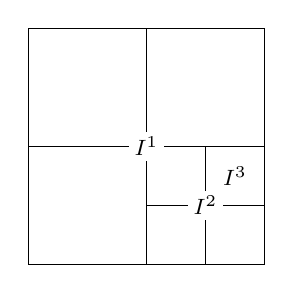
\begin{tikzpicture}[scale=1.5]
            \footnotesize
            \draw
                (0,0) rectangle (2,2)
                (1,0) -- ++(0,2)
                (0,1) -- ++(2,0)
                (1.5,0) -- ++(0,1)
                (1,0.5) -- ++(1,0)
            ;

            \node [fill=white,inner sep=2pt] at (1,1) {$I^1$};
            \node [fill=white,inner sep=2pt] at (1.5,0.5) {$I^2$};
            \node [fill=white,inner sep=2pt] at (1.75,0.75) {$I^3$};
        \end{tikzpicture}
        \caption{$k$-cells are compact.}
        \label{fig:kcellCompact}
    \end{figure}
    \begin{itemize}
        \item Argue by contradiction.
        \item Consider an open cover of the $k$-cell $I^1$. If it has a finite subcover, we're done. So suppose we have an open cover that doesn't have a finite subcover. Split the $k$-cell into $2^k$ chunks. At least one of the chunks $I^2$ must not have a finite subcover.
        \item Split that one into $2^k$ chunks. At least one of the chunks $I^3$ must not have a finite subcover.
        \item Continue.
        \item Thus, we have a decreasing family of $k$-cells, so by the previous result, their $\bigcap I^n\neq\emptyset$.
        \item Let $x\in\bigcap I^n$. Then the...
    \end{itemize}
    \item Heine-Borel theorem: Let $E\subset\R^k$. Then TFAE\footnote{The following are equivalent.}
    \begin{enumerate}
        \item $E$ is closed and bounded.
        \item $E$ is compact.
        \item Every infinite subset of $E$ has a limit point in $E$.
    \end{enumerate}
    \begin{itemize}
        \item ($1\Rightarrow 2$) $E$ closed and bounded implies $E$ is a closed subset of some $I_k$, so it's compact.
        \item ($2\Rightarrow 3$) Already done.
        \item ($3\Rightarrow 1$)
        \begin{itemize}
            \item Suppose $E$ not bounded. Then there is an infinite sequence of points in $E$ that never converges. Contradiction.
            \item Suppose $E$ is not closed. Then there exists a sequence of points in $E$ which "converges" to an $x_0\notin E$.
        \end{itemize}
    \end{itemize}
\end{itemize}



\section{Chapter 2: Basic Topology}
\emph{From \textcite{bib:Rudin}.}
\begin{itemize}
    \item \marginnote{11/6:}\textbf{Countable} (set $A$): A set $A$ that is in bijective correspondence with the set of all positive integers. \emph{Also known as} \textbf{enumerable}, \textbf{denumerable}.
    \item \textbf{At most countable} (set $A$): A set $A$ that is finite or countable.
    \item An alternative definition of an \textbf{infinite} set would be a set that is equivalent to one of its proper subsets.
    \item Theorem: Let $A$ be the set of all sequences whose elements are the digits 0 and 1. This set $A$ is uncountable.
    \begin{proof}
        Let $E=\{s_1,s_2,\dots\}$ be an arbitrary countable subset of $A$, where each $s_j$ is a sequence whose elements are the digits 0 and 1. Let $s$ be the sequence, the $n^\text{th}$ term of which is the opposite of the $n^\text{th}$ term of $s_n$ (i.e., if the $n^\text{th}$ term of $s_n$ is 0, we set the $n^\text{th}$ term of $s$ equal to 1). This guarantees that $s$ is distinct from each of the $s_j$, i.e., that $s\notin E$. It follows that $E\subsetneq A$, i.e., that every countable subset of $A$ is a proper subset of $A$. Therefore, $A$ must be uncountable (for otherwise $A$ would be a proper subset of $A$, a contradiction).
    \end{proof}
    \begin{itemize}
        \item The idea of this proof is called \textbf{Cantor's diagonalization process}.
        \item Since every real number can be represented as a binary sequence of numbers, i.e., $A\sim\R$, the reals are uncountable.
    \end{itemize}
    \item \textbf{Metric space}: A set $X$ such that with any two points $p,q\in X$, there is associated a real number $d(p,q)$ such that
    \begin{enumerate}
        \item $d(p,q)>0$ if $p\neq q$; $d(p,p)=0$.
        \item $d(p,q)=d(q,p)$.
        \item $d(p,q)\leq d(p,r)+d(r,q)$ for any $r\in X$.
    \end{enumerate}
    \item \textbf{Distance} (from $p\in X$ to $q\in X$, $X$ a metric space): The real number $d(p,q)$.
    \item \textbf{Distance function}: A function $d:X\times X\to\R$ that sends $(p,q)\mapsto d(p,q)$. \emph{Also known as} \textbf{metric}.
    \item Every subset of a metric space is a metric space in its own right under the same distance function.
    \item \textbf{Segment} (from $a$ to $b$): The set of all real numbers $x$ such that $a<x<b$. \emph{Denoted by} $\bm{(a,b)}$.
    \item \textbf{Interval} (from $a$ to $b$): The set of all real numbers $x$ such that $a\leq x\leq b$. \emph{Denoted by} $\bm{[a,b]}$.
    \item \textbf{$\bm{k}$-cell}: The set of all points $\x=(x_1,\dots,x_k)\in\R^k$ whose coordinates satisfy the inequalities $a_i\leq x_i\leq b_i$ where $a_i<b_i$ for each $1\leq i\leq k$.
    \begin{itemize}
        \item Note that a 1-cell is an interval and a 2-cell is a rectangle.
    \end{itemize}
    \item \textbf{Convex} (set $E$): A subset $E$ of $\R^k$ such that
    \begin{equation*}
        \lambda\x+(1-\lambda)\y \in E
    \end{equation*}
    for all $\x,\y\in E$ and $0<\lambda<1$.
    \begin{itemize}
        \item Balls and $k$-cells are both convex.
    \end{itemize}
    \item The segment $(a,b)$ is open as a subset of $\R^1$, but not open as a subset of $\R^2$.
    \item Since compactness is not relative, while it makes no sense to talk about \emph{open} or \emph{closed} metric spaces, it does make sense to talk about \emph{compact} metric spaces.
    \item \textbf{Weierstrass theorem}: Every bounded infinite subset of $\R^k$ has a limit point in $\R^k$.
    \item Theorem: Let $P$ be a nonempty perfect set in $\R^k$. Then $P$ is uncountable.
    \begin{proof}
        Since $P$ is nonempty and perfect, there exists a limit point of $P$. It follows that $P$ is infinite.\par
        Now suppose for the sake of contradiction that $P$ is countable, and denote the elements of $P$ by $\x_1,\x_2,\dots$. We now construct a sequence $\{V_n\}$ of neighborhoods, as follows. Let $V_1=N_r(\x_1)$. Clearly, $V_1\subset P$ since $\x_1\in P$. It follows that since $V_1$ is a neighborhood that $V_1$ contains infinitely many points of $P$. Now suppose inductively that $V_n$ has been constructed. Thus, by analogous conditions to those on $V_1$, we may let $V_{n+1}$ be a neighborhood such that (i) $\bar{V}_{n+1}\subset V_n$, (ii) $\x_n\notin\bar{V}_{n+1}$, and (iii) $V_{n+1}\cap P$ is nonempty. By (iii), we can continue on to construct $V_{n+2}$, and so on and so forth.\par
        Let $K_n=\bar{V}_n\cap P$. Since $\bar{V}_n$ is closed and bounded, $\bar{V}_n$ is compact. Additionally, since $\x_n\notin K_{n+1}$ for each $n$, no point of $P$ lies in $\bigcap_1^\infty K_n$. Thus, since each $K_n\subset P$, $\bigcap_1^\infty K_n$ is empty. But this contradicts our previous result that since each $K_n$ is nonempty, compact, and such that $K_n\supset K_{n+1}$, $\bigcap_1^\infty K_n$ is nonempty.
    \end{proof}
    \item Corollary: Every interval $[a,b]$ is uncountable. In particular, $\R$ is uncountable.
    \item \textbf{Cantor set}: The set resulting from the following construction. Let $E_0=[0,1]$. Remove the segment $(1/3,2/3)$, so that $E_1=[0,1/3]\cup[1/3,2/3]$. Now remove the middle third of these two intervals to create $E_2$. Continue on indefinitely.
    \begin{itemize}
        \item This is a perfect set in $\R^1$ which contains no segment.
    \end{itemize}
    \item \textbf{Separated} (sets $A,B$): Two subsets $A,B$ of a metric space $X$ such that $A\cap\bar{B}$ and $\bar{A}\cap B$ are empty.
    \item \textbf{Connected} (set $E$): A set $E$ that is not the union of two nonempty separated sets.
    \item Separated sets are disjoint, but disjoint sets are not necessarily separated (consider $[0,1]$ and $(1,2)$).
    \item A subset $E$ of $\R^1$ is connected if and only if it has the following property: If $x,y\in E$ and $x<z<y$, then $z\in E$.
\end{itemize}




\end{document}